\chapter{本模板遵循的排版与论文写作的格式}
\label{cha:format}
本章将介绍本模板遵循的排版及格式。
\section{排版}
\label{sec:composition}
在介绍本模板的排版和格式之前,本章首先介绍一些基本的概念,如图 \ref{fig:composition_general} 所示。图 \ref{fig:composition_general} 中的英文为geometry宏包中的参数,纸张默认设置为A4大小,body或total body为正文内容所在区域。重要的参数有7个,分别是:top、bottom、left、right、headheight、headsep、footskip。top和bottom分别为上边距和下边距,本模板按照word默认设置为1英寸;left和right分别为左边距和右边距,本模板按照word默认设置为1.25英寸;headsep为页眉(横线)与正文区域的距离,本模板按照word默认设置为0.2英寸;headheight为页眉内容的高度,本模板按照word默认设置页眉顶端距离页面边界1.5 cm,计算得到headheight为0.532 cm;footskip为页脚内容的高度,本模板按照word默认设置页脚底部距离页面边界1.75 cm,计算得到footskip为0.79 cm。
\begin{figure}[H] 
	\centering
	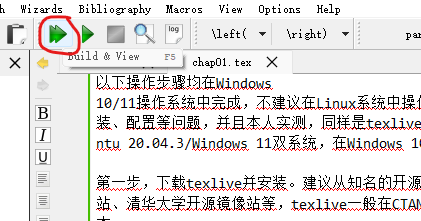
\includegraphics[width=0.6\textwidth]{image/chap01/f5.png}
	\caption{Build \& View}
	\label{fig:f5}
\end{figure}

每一章的标题采用小二号黑体,居中;节标题采用小三号黑体

